% !TEX root = ../main.tex
\lecture{4}{2026-10-06}{Arten von Informationssysteme}

\section{Informationssysteme: Einsatzgebiete}
\subsection{Enterprise-Resource-Planning ERP}
\begin{definition}
    [ERP] Integrierte Interne Anwendungssysteme zur Koordination interner Prozesse.
\end{definition}

\begin{itemize}
    \item Geschäftsprozesse von Lieferanten bis Kunden unterstützen 
    \item Bereiche:
    \begin{itemize}
        \item Fertigung Produktion
        \item Finanz und Rechnungswesen (Auswicklung )
        \item Vertrieb und Marketing
        \item Personalwesen
    \end{itemize}
\end{itemize}

\subsection{Suply-Chain-Management SCM}

\begin{definition}
    [SCM] Automatisierung von Informationsaustausch zwischen Unternehmen und seinen Lieferanten/Kunden
\end{definition}
\subsubsection{Nutzen}
SCMs optimieren Lieferketten, sodass die Verweilzeit von Waren im Lager massiv reduziert werden. Die Produktion kann schnell auf die Nachfrage reagieren und prognostizieren.
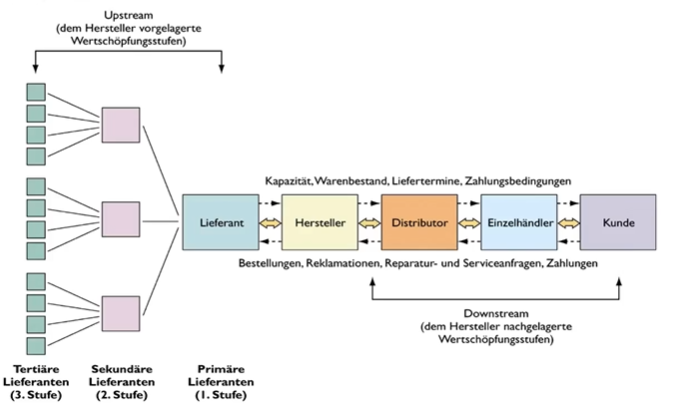
\includegraphics[width=\textwidth,height=0.7\textheight,keepaspectratio]{figures/SCM.png}


\subsection{Customer Relationship Management CRM}

\begin{definition}
    [CRM] System zur Analyse von Kunden Beziehungen aus verschiedenen Perspektiven. Daten aus Vertrieb, Marketing und Kundenservice.
\end{definition}


\subsection{Wissensmanagement}
\begin{definition}
    [Wissensmanagement] Systeme, die den Erwerb, Erfassung, Speicherung und Weitergabe von Fachwissen und häufiggestellte Fragen verwalten. 
\end{definition}

\subsection{Content Management Systeme CMS}
\begin{definition}
    [CMS] Systeme zur Verwaltung und Unterstützung kollaborativer Erarbeitung von Inhalte (Texte, Webseiten, Bilder, Videos, Dokumente etc.) 
\end{definition}

\subsection{Fazit}

\begin{itemize}
    \item Informationssysteme Unterstützen aktuell alle Bereiche der Wertschöpfung
    \item Aus ihren Einsatz können Daten gesammelt werden für die weitere Optimierung durch analytische IS
\end{itemize}

\section{Informationssysteme: Wertschöpfungsphasen}

\subsection{Funktionsweise}


\begin{enumerate}
    \item Eingabe oder Extraktion
    \begin{itemize}
        \item Daten kommen aus den internen Prozesse oder externe Quellen
    \end{itemize}
    \item Aufbereitung 
    \begin{itemize}
        \item Nach
    \end{itemize}
\end{enumerate}
